%==============================常用宏包、环境==============================%
\documentclass[twocolumn,a4]{article}
\usepackage{xeCJK} % For Chinese characters
\usepackage{amsmath, amsthm}
\usepackage{listings,xcolor}
\usepackage{geometry} % 设置页边距
\usepackage{fontspec}
\usepackage{graphicx}
\usepackage{float} %设置图片浮动位置的宏包
\usepackage{subfigure} %插入多图时用子图显示的宏包
\usepackage{fancyhdr} % 自定义页眉页脚
\setsansfont{Consolas} % 设置英文字体
\setmonofont[Mapping={}]{Consolas} % 英文引号之类的正常显示,相当于设置英文字体
\geometry{left=1cm,right=1cm,top=2cm,bottom=0.5cm} % 页边距
\setlength{\columnsep}{30pt}
% \setlength\columnseprule{0.4pt} % 分割线
%==============================常用宏包、环境==============================%

%==============================页眉、页脚、代码格式设置==============================%
% 页眉、页脚设置
\pagestyle{fancy}
% \lhead{CUMTB}
\lhead{\CJKfamily{hei} 泡泡猿专用模板}
\chead{}
% \rhead{Page \thepage}
\rhead{\CJKfamily{hei} 第 \thepage 页}
\lfoot{} 
\cfoot{}
\rfoot{}
\renewcommand{\headrulewidth}{0.4pt} 
\renewcommand{\footrulewidth}{0.4pt}

% 代码格式设置
\lstset{
    language    = c++,
    numbers     = left,
    numberstyle = \tiny,
    breaklines  = true,
    captionpos  = b,
    tabsize     = 4,
    frame       = shadowbox,
    columns     = fullflexible,
    commentstyle = \color[RGB]{0,128,0},
    keywordstyle = \color[RGB]{0,0,255},
    basicstyle   = \small\ttfamily,
    stringstyle  = \color[RGB]{148,0,209}\ttfamily,
    rulesepcolor = \color{red!20!green!20!blue!20},
    showstringspaces = false,
}
%==============================页眉、页脚、代码格式设置==============================%

%==============================标题和目录==============================%
\title{\CJKfamily{hei} \bfseries 泡泡猿ACM模板}
\author{Rand0w \& REXWIND \& Dallby}
\renewcommand{\today}{\number\year 年 \number\month 月 \number\day 日}

\begin{document}\small
\begin{titlepage}
\maketitle
\begin{figure}[H] %H为当前位置,!htb为忽略美学标准,htbp为浮动图形
\centering %图片居中
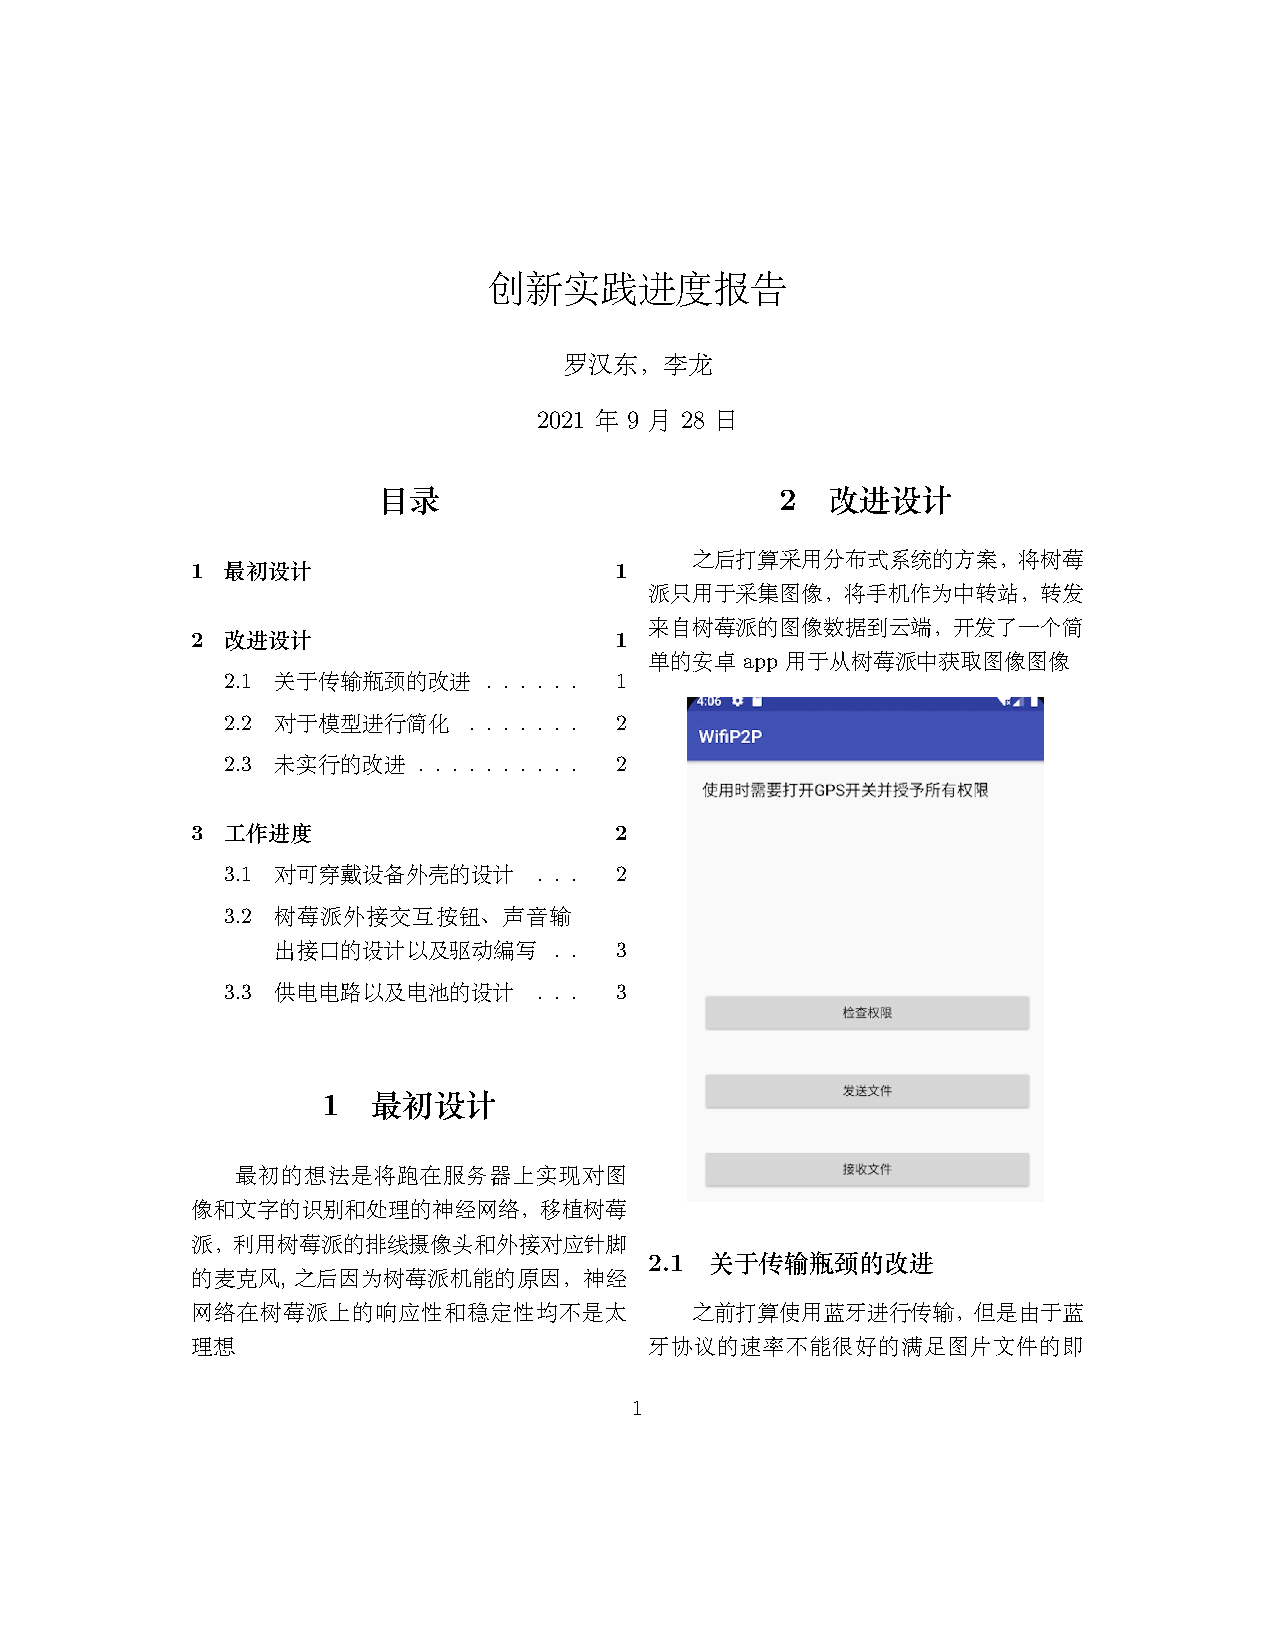
\includegraphics[width=0.7\textwidth]{1.jpg} %插入图片,[]中设置图片大小,{}中是图片文件名
\end{figure}
\end{titlepage}

\newpage
\pagestyle{empty}
\renewcommand{\contentsname}{目录}
\tableofcontents
\newpage\clearpage
\newpage
\pagestyle{fancy}
\setcounter{page}{1}   %new page
%==============================标题和目录==============================%

%==============================正文部分==============================%
\section{头文件}
\subsection{头文件(Rand0w)}
\begin{lstlisting}
#include <bits/stdc++.h>
//#include <bits/extc++.h>
//using namespace __gnu_pbds;
//using namespace __gnu_cxx;
using namespace std;
#pragma optimize(2)
//#pragma GCC optimize("Ofast,no-stack-protector")
//#pragma GCC target("sse,sse2,sse3,ssse3,sse4,popcnt,abm,mmx,avx,avx2,tune=native")
#define rbset(T) tree<T,null_type,less<T>,rb_tree_tag,tree_order_statistics_node_update>
const int inf = 0x7FFFFFFF;
typedef long long ll;
typedef double db;
typedef long double ld;
template<class T>inline void MAX(T &x,T y){if(y>x)x=y;}
template<class T>inline void MIN(T &x,T y){if(y<x)x=y;}
namespace FastIO
{
char buf[1 << 21], buf2[1 << 21], a[20], *p1 = buf, *p2 = buf, hh = '\n';
int p, p3 = -1;
void read() {}
void print() {}
inline int getc()
{
return p1 == p2 && (p2 = (p1 = buf) + fread(buf, 1, 1 << 21, stdin), p1 == p2) ? EOF : *p1++;
}
inline void flush()
{
fwrite(buf2, 1, p3 + 1, stdout), p3 = -1;
}
template <typename T, typename... T2>
inline void read(T &x, T2 &... oth)
{
int f = 0;x = 0;char ch = getc();
while (!isdigit(ch)){if (ch == '-')f = 1;ch = getc();}
while (isdigit(ch)){x = x * 10 + ch - 48;ch = getc();}
x = f ? -x : x;read(oth...);
}
template <typename T, typename... T2>
inline void print(T x, T2... oth)
{
if (p3 > 1 << 20)flush();
if (x < 0)buf2[++p3] = 45, x = -x;
do{a[++p] = x % 10 + 48;}while (x /= 10);
do{buf2[++p3] = a[p];}while (--p);
buf2[++p3] = hh;
print(oth...);
}
} // namespace FastIO
#define read FastIO::read
#define print FastIO::print
#define flush FastIO::flush
#define spt fixed<<setprecision
#define endll '\n'
#define mul(a,b,mod) (__int128)(a)*(b)%(mod) 
#define pii(a,b) pair<a,b>
#define pow powmod
#define X first
#define Y second
#define lowbit(x) (x&-x)
#define MP make_pair
#define pb push_back
#define pt putchar
#define yx_queue priority_queue
#define lson(pos) (pos<<1)
#define rson(pos) (pos<<1|1)
#define y1 code_by_Rand0w
#define yn A_muban_for_ACM
#define j1 it_is just_an_eastegg
#define lr hope_you_will_be_happy_to_see_this
#define int long long
#define rep(i, a, n) for (register int i = a; i <= n; ++i)
#define per(i, a, n) for (register int i = n; i >= a; --i)
const ll llinf = 4223372036854775851;
const ll mod = (0 ? 1000000007 : 998244353);
ll pow(ll a,ll b,ll md=mod) {ll res=1;a%=md; assert(b>=0); for(;b;b>>=1){if(b&1)res=mul(res,a,md);a=mul(a,a,md);}return res;}
const ll mod2 = 999998639;
const int m1 = 998244353;
const int m2 = 1000001011;
const int pr=233;
const double eps = 1e-7;
const int maxm= 1;
const int maxn = 510000;
void work()
{
	
}
signed main()
{
   #ifndef ONLINE_JUDGE
   //freopen("in.txt","r",stdin);
	//freopen("out.txt","w",stdout);
#endif
	//std::ios::sync_with_stdio(false);
	//cin.tie(NULL);
	int t = 1;
	//cin>>t;
	for(int i=1;i<=t;i++){
		//cout<<"Case #"<<i<<":"<<endll;
		work();
	}
	return 0;
}
\end{lstlisting}
\subsection{头文件(REXWind)}
\begin{lstlisting}
cout<<"hello<<endl;
\end{lstlisting}
\subsection{头文件(Dallby)}
\begin{lstlisting}
#include<bits/stdc++.h>
cout<<"hello<<endl;
\end{lstlisting}


%==============================正文部分==============================%
\end{document}